\begin{frame}
  \frametitle{What is a Molten Salt Reactor (MSR)?}
	\begin{itemize}
	  \item Advanced nuclear reactor fueled by fissile
		material dissolved in a molten salt mixture
	  \item In most MSR designs, the fuel salt mixture doubles as the primary coolant for the
        reactor
	  \item Both thermal- and fast-spectrum configurations are viable
	\end{itemize}
	\begin{figure}
	  \centering
	  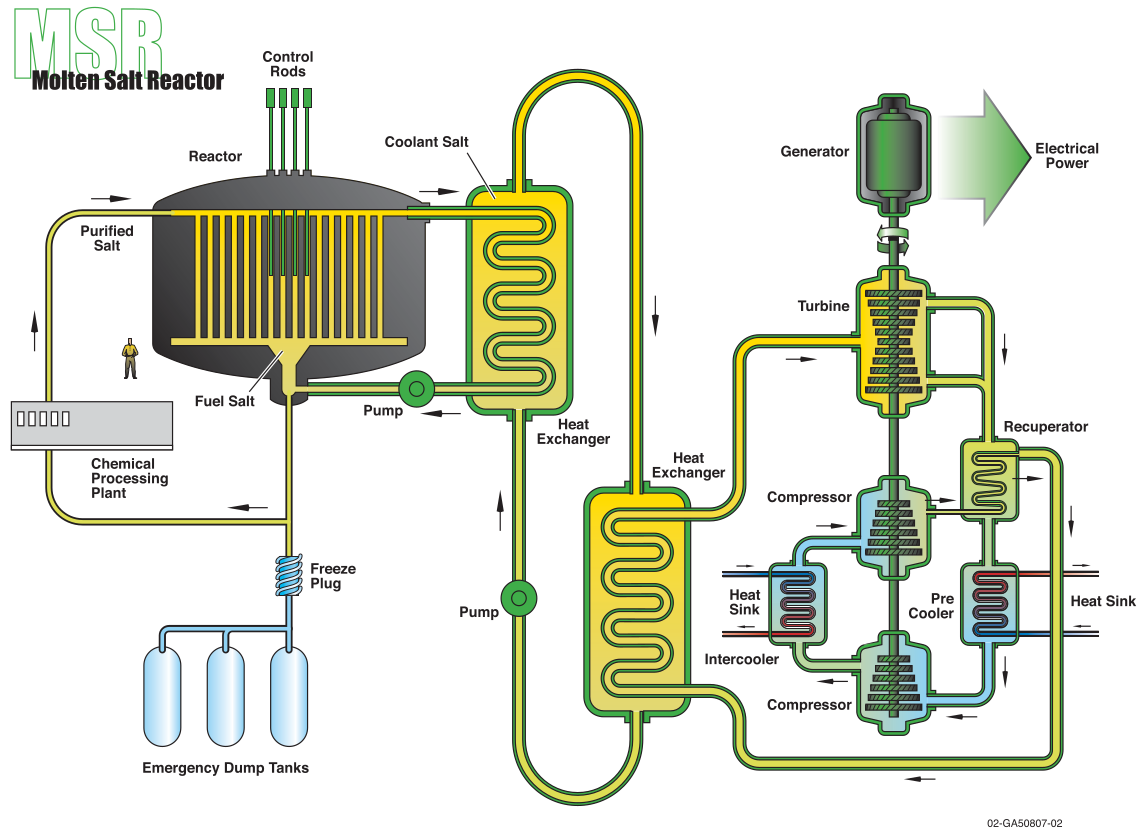
\includegraphics[width=.5\textwidth]{./images/msr}
      \caption{Schematic diagram of a general channel-type MSR concept \cite{doe_technology_2002}.}
	  \label{fig:msr}
	\end{figure}
\end{frame}

\begin{frame}
  \frametitle{What is a Molten Salt Reactor (MSR)?}
  \textbf{Advantages of MSRs over other reactor types}
  \begin{itemize}
    \item Robust passive safety
      \begin{itemize}
        \item strong temperature feedback
        \item large thermal margin to boiling
      \end{itemize}
    \item Freeze plugs drains fuel salt into containment tanks under emergency situations
    \item Online refueling and reprocessing can:
      \begin{itemize}
        \item reduce reactor downtime
        \item reduce required fissile inventory in reactor at any given time
        \item reduce transuranic waste produced
        \item allow for $^{233}$U breeding from $^{232}$Th
      \end{itemize}
    \item Viable as fast-spectrum breeder/burner reactor
    \item Can provide high-temperature heat for industrial heat applications
  \end{itemize}
\end{frame}

\begin{frame}
  \frametitle{Molten Salt Reactor Modeling \& Simulation}
  \textbf{While modeling MSRs is not necessarily more difficult than modeling solid-fueled
  reactors, we must adapt our software tools to accurately model phenomena unique to MSRs.}\\

  \textbf{Phenomena which pose challenges for MSR modeling}
  \begin{itemize}
	\item Strong multiphysics interactions involving neutron flux, temperature, and flow in the
      reactor core
	  \begin{itemize}
		\item Strong temperature feedback due to thermal expansion of liquid fuel salt
		\item Movement of \gls{DNP} along primary coolant loop
        \item Advection-dominated heat transfer
	  \end{itemize}
    \item Loss of delayed neutrons to out-of-core decay
    \item Complex turbulent flow effects in MSRs with wide flow channels
  \end{itemize}
\end{frame}

